%% LyX 2.0.2 created this file.  For more info, see http://www.lyx.org/.
%% Do not edit unless you really know what you are doing.
\documentclass[12pt,letterpaper,english,12pt,english,openany,letterpaper,pagesize]{scrbook}
\usepackage[T1]{fontenc}
\usepackage[latin9]{inputenc}
\setlength{\parskip}{\medskipamount}
\setlength{\parindent}{0pt}
\usepackage{float}
\usepackage{amsthm}
\usepackage{amsmath}
\usepackage{graphicx}
\usepackage{setspace}
\onehalfspacing

\makeatletter

%%%%%%%%%%%%%%%%%%%%%%%%%%%%%% LyX specific LaTeX commands.
\pdfpageheight\paperheight
\pdfpagewidth\paperwidth


%%%%%%%%%%%%%%%%%%%%%%%%%%%%%% User specified LaTeX commands.
%\documentclass[12pt,spanish,fleqn,openany,letterpaper,pagesize]{scrbook}

%\usepackage[ansinew]{inputenc}
%\usepackage[spanish]{babel}
\usepackage{fancyhdr}
\usepackage{epsfig}
\usepackage{epic}
\usepackage{eepic}
\usepackage{amsmath}
\usepackage{threeparttable}
\usepackage{amscd}
\usepackage{here}
\usepackage{graphicx}
\usepackage{lscape}
\usepackage{tabularx}
\usepackage{subfigure}
\usepackage{longtable}


\usepackage{rotating} %Para rotar texto, objetos y tablas seite. No se ve en DVI solo en PS. Seite 328 Hundebuch
                        %se usa junto con \rotate, \sidewidestable ....


\renewcommand{\theequation}{\thechapter-\arabic{equation}}
\renewcommand{\thefigure}{\textbf{\thechapter-\arabic{figure}}}
\renewcommand{\thetable}{\textbf{\thechapter-\arabic{table}}}


\pagestyle{fancyplain}%\addtolength{\headwidth}{\marginparwidth}
\textheight22.5cm \topmargin0cm \textwidth16.5cm
\oddsidemargin0.5cm \evensidemargin-0.5cm%
\renewcommand{\chaptermark}[1]{\markboth{\thechapter\; #1}{}}
\renewcommand{\sectionmark}[1]{\markright{\thesection\; #1}}
\lhead[\fancyplain{}{\thepage}]{\fancyplain{}{\rightmark}}
\rhead[\fancyplain{}{\leftmark}]{\fancyplain{}{\thepage}}
\fancyfoot{}
\thispagestyle{fancy}%


\addtolength{\headwidth}{0cm}
\unitlength1mm %Define la unidad LE para Figuras
%\mathindent0cm %Define la distancia de las formulas al texto,  fleqn las descentra
\marginparwidth0cm
\parindent0cm %Define la distancia de la primera linea de un parrafo a la margen

%Para tablas,  redefine el backschlash en tablas donde se define la posici\'{o}n del texto en las
%casillas (con \centering \raggedright o \raggedleft)
\newcommand{\PreserveBackslash}[1]{\let\temp=\\#1\let\\=\temp}
\let\PBS=\PreserveBackslash

%Espacio entre lineas
\renewcommand{\baselinestretch}{1.1}

%Neuer Befehl f\"{u}r die Tabelle Eigenschaften der Aktivkohlen
\newcommand{\arr}[1]{\raisebox{1.5ex}[0cm][0cm]{#1}}

%Neue Kommandos
\usepackage{resources/Befehle}


%Trennungsliste
\hyphenation {Reaktor-ab-me-ssun-gen Gas-zu-sa-mmen-set-zung
Raum-gesch-win-dig-keit Durch-fluss Stick-stoff-gemisch
Ad-sorp-tions-tem-pe-ra-tur Klein-schmidt
Kohlen-stoff-Mole-kular-siebe Py-rolysat-aus-beu-te
Trans-port-vor-gan-ge}

%\pagenumbering{roman}
%\let\myTOC\tableofcontents
%\renewcommand\tableofcontents{%
%\myTOC
%\clearpage
%\pagenumbering{arabic}
%}

\makeatother

\usepackage{babel}
\begin{document}

\chapter{Mesh smoothing based on curvature flow operator in a diffusion equation\label{sub:Laplacian-Smooth}}

This work was accepted as part of the software Blender \cite{blender},
an open source 3D application for modeling, animation, rendering,
compositing, video editing and game creation. The work was supported
by an awarded internship of the Google Summer of Code 2012 program,
administered for Google Inc.


\section{Synopsis}

Computer graphics objects reconstructed from real world contain undesirable
noise. A Mesh smoothing removes undesirable noise while still preserving
desirable geometric and shape of the original model.

This project improving the mesh smoothing tools in blender, based
on curvature flow operator in a diffusion equation.

This project allows working with hybrid meshes composed by triangles
and quads based on Laplacian operator proposed by Pinz�n and Romero
\cite{Pinzon2013}.


\section{Benefits to Blender}

This project proposes a new and robust mesh smoothing tool for blender
user that require improves the appearance of surfaces models.

New methods to scan computer graphics objects using the Kinect ZCam
within Blender, need to remove the noise present at the time of capture.

This mesh smoothing method produce higher quality results without
shrinkage. The smoothing tool current collapses the mesh after several
iterations.

This mesh smoothing method permit uses a hard and soft constraints
on the positions of the points in the mesh to maintain control over
the shape.

This mesh smoothing method can help to remove noise generated during
the sculpting, without removal the desired details of the model.


\section{Deliverables }

A new and robust mesh smoothing tool for Blender. 

Some pages of documentation to be included in the manual.

A technical document for developers to improve the method in the future.

A tutorial explaining the use of the tool.


\section{Project Details }

The project would divide into four parts:

To implement mesh smoothing algorithm based on curvature flow operator
in a diffusion equation for blender geometric structures.
\begin{enumerate}
\item Initialize data and necessary structures. 
\item Compute the Laplacian Matrix. 
\item Define the sparse linear system.
\item Solving the sparse linear system, we can use a preconditioned bi-conjugated
gradient numerical library. 
\end{enumerate}
Integrate or use numerical library present in Blender to solve sparse
linear system

Generation of the documentation and tutorials.


\section{Project Schedule}
\begin{itemize}
\item 3 weeks: Understanding the Blender source code and identify the key
points for the project.
\item 1 week: Define the data structures necessary to work with the architecture
of blender.
\item 1 week: Implement methods for the initial configuration needed for
the smoothing algorithm. Implement the method that calculates the
Laplacian matrix.
\item 2 week: Integrate or use numerical library.
\item 2 week: Define the sparse linear system and implement the method to
solve sparse linear system.
\item 3 weeks: Define and implement graphical user integration.
\item 2 weeks: Testing the tool.
\item 3 weeks: Generation of the documentation and tutorials
\end{itemize}

\section{Mesh Smoothing}

A common way to attenuate noise in a polygonal mesh is through a diffusion
process \cite{Taubin1995,Desbrun1999}. Laplacian smooth techniques
over a diffusion process allow a proper noise reduction on the mesh
surface with minimal shape changes, while still preserving a desirable
geometry as well as the original shape. The simple idea is that the
vertices are moved in the direction of the Laplacian when we use the
cotangent version the vertices are moved in the direction of the curvature
flow. The complexity of Laplacian smoothing can be linear in time
and space with a fast convergence and the diffusion process can attenuate
noise with only one iteration due the sparseness of the laplacian
operator.

\noindent 
\begin{equation}
\frac{\partial V}{\partial t}=\lambda L\left(V\right)\label{eq:diffusion_process}
\end{equation}


Where L is the Laplacian matrix defined in equation \ref{eq:LaplacianMatrixForSmoothing}
for meshes composed by triangles or quads with different size or irregular
sampling. $\lambda$ is a scalar that control the diffusion process,
and smoothing factor.

The equation \ref{eq:diffusion_process} can be linearly approximated
using implicit integration with a Laplacian Operator version of TQLBO,
the use of implicit integration permit the system to be more stability.

\begin{equation}
\left(I-\lambda dtL\right)V^{n+1}=V^{n}\label{eq:LaplacianSmoothLinearEquationSystem}
\end{equation}


To permit the user to define the region of interest where the laplacian
smooth to be applied, we add a diagonal matrix $W_{p}$ to equation
\ref{eq:LaplacianSmoothLinearEquationSystem} where the every element
in the diagonal correspond to the weight for every vertex.

\noindent \begin{center}
$\left(I-\lambda dtW_{p}L\right)V^{n+1}=V^{n}$
\par\end{center}

For non-close meshes or meshes with holes is not possible to compute
the curvature flow. For this reason the system smooth the edges differently
within the diffusion process. The boundaries are treated as a one-dimensional
curve. In a curve the Laplacian is defined as the weighted difference
between the vertex and the two immediate neighbors, thus ensures the
curve maintained its original form as much as possible. We define
a Laplacian for mesh smoothing as a matrix equation.

\noindent \begin{center}
\begin{equation}
L(i,j)=\begin{cases}
-\frac{1}{2A_{i}}w_{ij} & \mbox{if }j\in N(v_{i})\wedge v_{i}\notin\mbox{Boundary}\\
\frac{1}{2A_{i}}\underset{j\in N\left(v_{i}\right)}{\sum}w_{ij} & \mbox{if }i=j\wedge v_{i}\notin\mbox{Boundary}\\
-e_{ij} & \mbox{if }j\in N(v_{i})\wedge\left\{ v_{i},v_{j}\right\} \in\mbox{Boundary}\\
\frac{2}{E_{i}}\underset{j\in N\left(v_{i}\right)}{\sum}e_{ij} & \mbox{if }i=j\wedge\left\{ v_{i},v_{j}\right\} \in\mbox{Boundary}\\
0 & \mbox{otherwise}
\end{cases}\label{eq:LaplacianMatrixForSmoothing}
\end{equation}

\par\end{center}

Where $L$ is a $n\times n$ matrix, $n$ is the number of vertices
of a given mesh $M$, $w_{ij}$ is the TQLBO defined in equation (\ref{PAPER:eq:TQLBO_wij}),
$N\left(v_{i}\right)$ is the 1-ring neighborhood with shared face
to $v_{i}$, $e_{ij}=\frac{1}{\left\Vert v_{i}-v_{j}\right\Vert }$
is the inverse length of the edge between vertices $\left\{ v_{i},v_{j}\right\} $,
$E_{i}=\underset{j\in N\left(v_{i}\right)}{\sum}e_{ij}$. $A_{i}$
is the ring area around $v_{i}$.


\section{Results and Conclusions}

The user interface developed to this tool for the software Blender
can be seen in figure \ref{fig:Interface-LaplacianSmoothing}. This
tool allows to set the parameters of $\lambda$ for interior points
and boundaries. Allows to configure soft constraints using weights
defined by vertices in ``Vertex Group'', and allows you to set strong
constraints applying the algorithm independently of axis X, Y or Z.

\begin{figure}[H]
\noindent \begin{centering}
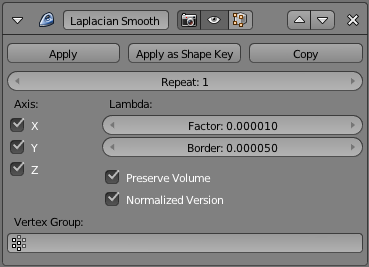
\includegraphics{resources/figs/Apinzonf_Diagram_Modifier_Panel}
\par\end{centering}

\caption{\label{fig:Interface-LaplacianSmoothing}Panel inside blender user
interface of the Laplacian Smooth modifier tool.}
\end{figure}


The tool developed can set the parameter $\lambda dt$ of equation
\ref{eq:LaplacianSmoothLinearEquationSystem}. Using a small Lambda
factor ($\lambda<1.0$), you can remove noise from the shape without
affecting desirable geometry (see figure \ref{fig:Factor-LaplacianSmoothing}.b).
Using a large Lambda factor ($\lambda>1.0$) you get smoothed versions
of the shape at the cost of losing fine geometry details (see figure
\ref{fig:Factor-LaplacianSmoothing}.c and \ref{fig:Factor-LaplacianSmoothing}.d).

\begin{figure}[H]
\noindent \begin{centering}
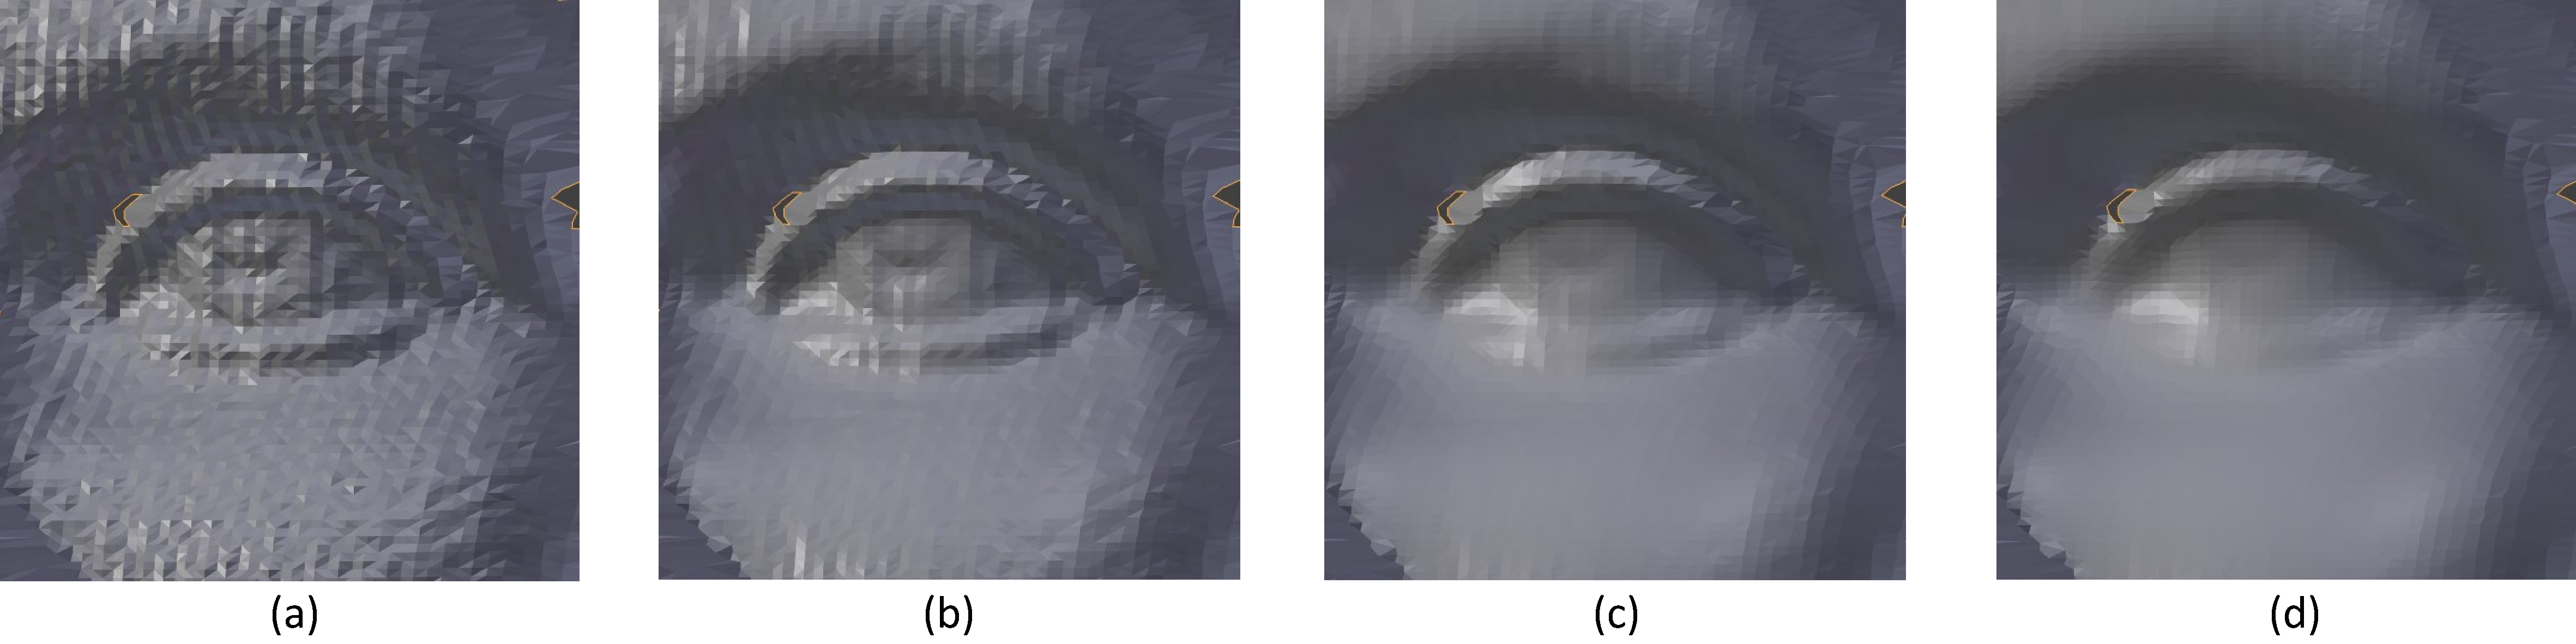
\includegraphics[width=1\textwidth]{resources/figs/LaplacianSmoothingFactor}
\par\end{centering}

\caption{\label{fig:Factor-LaplacianSmoothing}Noise attenuation in face model
with Laplacian smoothing tool using only one iteration and changing
$\lambda$. (a) Original Model. (b) Smoothing $\lambda=0.5$. (c)
Smoothing $\lambda=2.5$ (d) Smoothing with $\lambda=5.0$. }
\end{figure}


The user can smooth the boundaries configuring the parameter ``\textsl{Border}\textquotedbl{},
seen in figure \ref{fig:Interface-LaplacianSmoothing}. Boundaries
are treated differently. There is no way to calculate the curvature
flow on them. For this reason the Lambda factor ``$Border$'' just
smooths them. The change of this parameter and the results seen in
figure \ref{fig:Border-LaplacianSmoothing}, in the figure you can
see how the boundary inside the red circle is smoothing.

\begin{figure}[H]
\noindent \begin{centering}
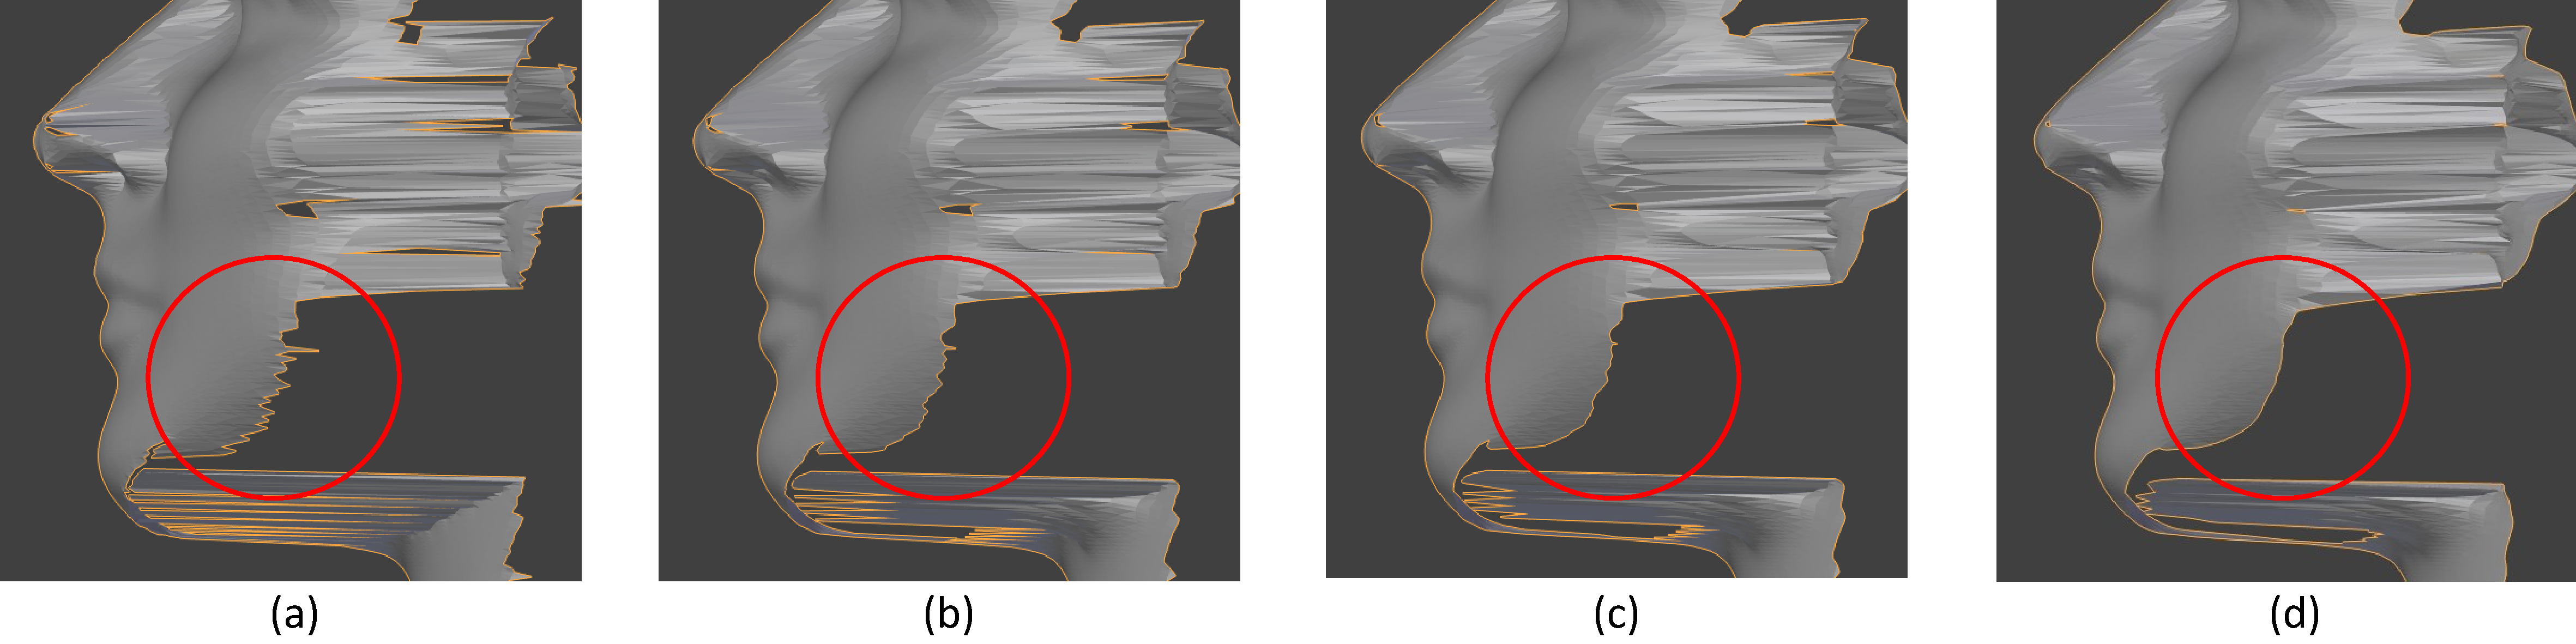
\includegraphics[width=1\textwidth]{resources/figs/LaplacianSmoothingBoundary}
\par\end{centering}

\caption{\label{fig:Border-LaplacianSmoothing} Smoothing boundary changing
$\lambda_{Border}$ factor. (a) Original Model. (b) Smoothing $\lambda_{Border}=1.0$.
(c) Smoothing $\lambda_{Border}=2.5$ (d) Smoothing with $\lambda_{Border}=10.0$. }
\end{figure}


The tool allows the user to add soft constraints using weights for
each vertex, this allows to define regions of interest where you want
to apply the algorithm in the figure \ref{fig:VertexGroup-LaplacianSmoothing}.c
defined in red region where you want it applied the algorithm the
results are shown in figure \ref{fig:VertexGroup-LaplacianSmoothing}.d
where only were smoothed vertices in the red region.

\begin{figure}[H]
\noindent \begin{centering}
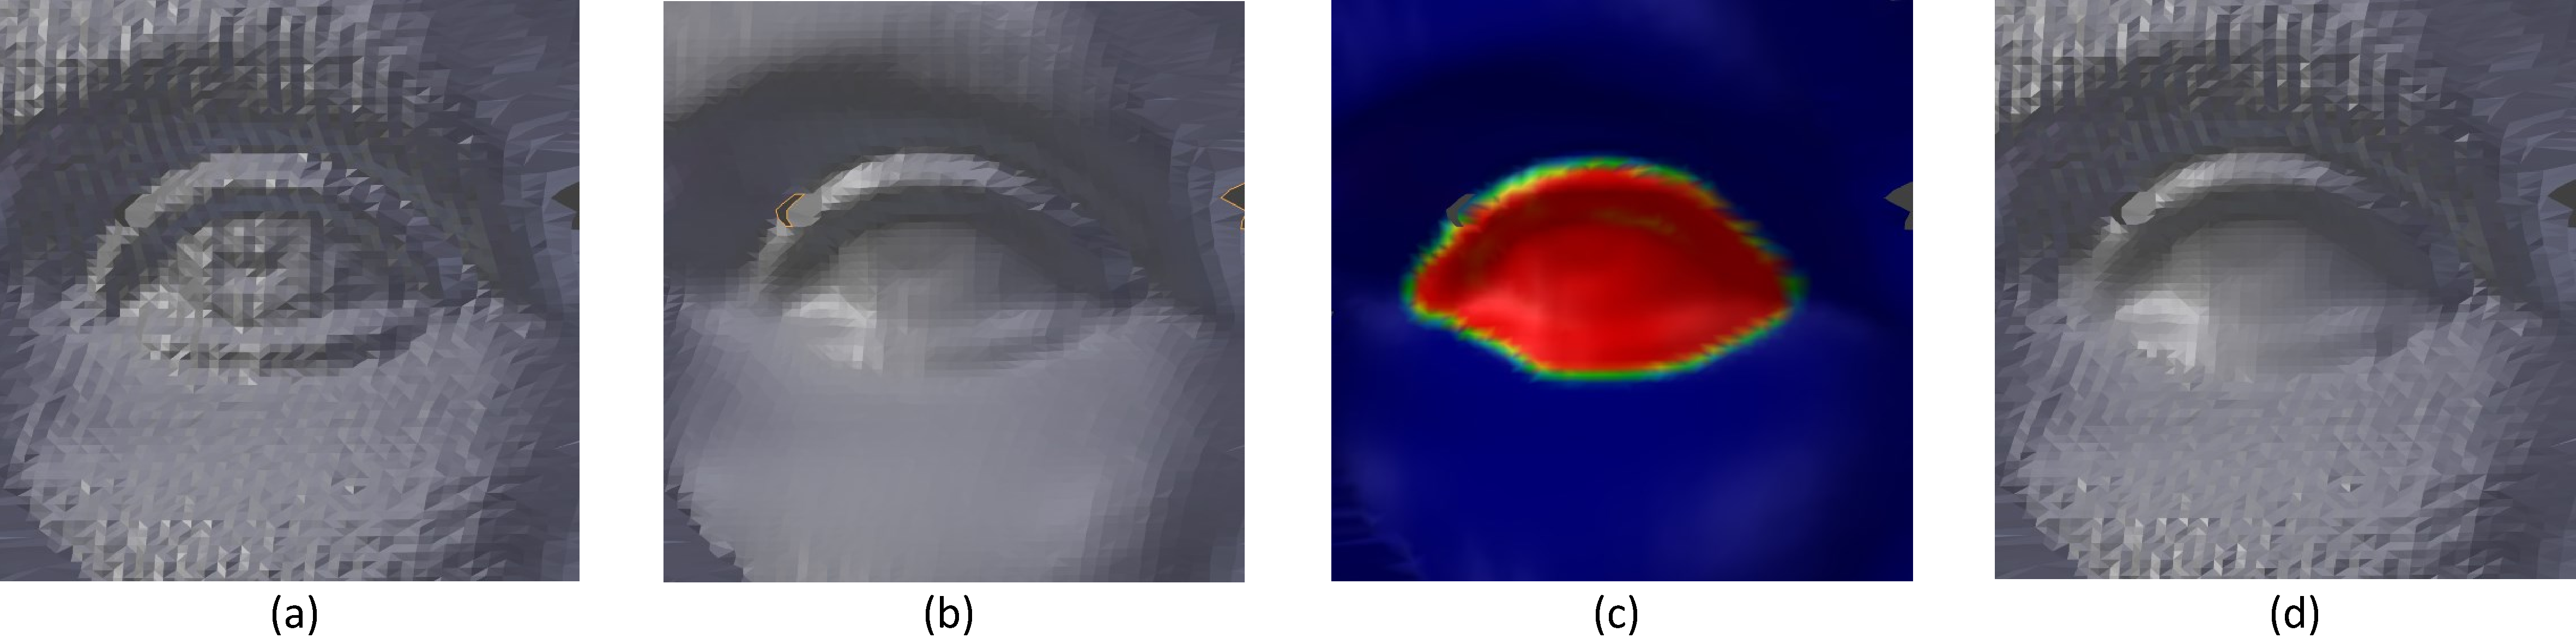
\includegraphics[width=1\textwidth]{resources/figs/LaplacianSmoothingVertecGroup}
\par\end{centering}

\caption{\label{fig:VertexGroup-LaplacianSmoothing}Use of weights per vertex
to constrain the effect of mesh smoothing. (a) Original Model. (b)
Smoothing with $\lambda=1.5$ (c) red vertices $weight=1.0$, blue
vertices $weight=0.0$. (d) Smoothing with $\lambda=2.5$. Red vertices
were only smoothing. }
\end{figure}


Module was developed as a tool for Blender software to remove noise
in the most efficient way as they had been doing.

The methods proposed in the art to remove noise, they could only be
applied if the mesh was composed only by triangles, with the developed
tool artists can now remove the noise of their models composed of
triangles and quadrangles.
\end{document}
